\documentclass[xcolor=pdftex,dvipsnames,table,numbers,hyperref={pdfpagelabels=false},compress]{beamer}
%\usepackage{requiredPackage}
\usepackage{amsmath}
\usepackage{graphicx}
\usepackage{amsfonts}
\usepackage{amssymb}

\usepackage{tabularx}
\usepackage{epstopdf}
\usepackage{overpic}
\usepackage{url}
\usepackage{calrsfs}
\usepackage{mathrsfs}
\usepackage{epsfig}
\usepackage{cancel}
\usepackage{changepage}

\usepackage{tikz}
\usepackage[customcolors]{hf-tikz} 

\usepackage{lmodern}
%\usepackage{mystyle}
\usepackage{subfig}
\usepackage{pifont}
\usepackage{tabu}
\usepackage{xcolor}
\usepackage{algorithm}
\usepackage{algpseudocode}
%\usepackage{enumitem}
\usepackage{remreset}
\usepackage{etoolbox}
\usepackage{comment} % end and begin comment
%\usepackage{dtklogos} 
\usepackage{listings}
\lstset{breaklines=true} 

\newcommand{\gline}{\textcolor{gray}{\hline}}
\newcommand{\cmark}{\ding{51}}%
\newcommand{\xmark}{\ding{55}}%
\newcommand{\gcheck}{\textcolor{blue}{\Large \cmark}}
\newcommand{\rcross}{\textcolor{red}{\Large \xmark}}
\newcommand{\tkt}{\tilde{K}_\theta}
\newcommand{\kt}{K_\theta}
\newcommand{\ind}{\overset{ind}{\sim}}
\newcommand{\plim}{\overset{p}{\rightarrow}}
\newcommand{\cx}{\frac {X'X}n}
\newcommand{\cz}{\frac {Z'Z}n}
\newcommand{\ccz}{\frac {Z'Z}n - \Sigma_A}
\newcommand{\czy}{\frac {Z'y}n}
\newcommand{\cyz}{\frac {y'Z}n}
\newcommand{\cxy}{\frac {X'y}n}
\newcommand{\cyx}{\frac {y'X}n}
\newcommand{\myitem}{\vskip3mm \item}

\newcommand{\calS}{{\cal S}}
\newcommand{\calA}{{\cal A}}
\newcommand{\calK}{{\cal K}}
\newcommand{\calX}{{\cal X}}
\newcommand{\calD}{{\cal D}}
\newcommand{\calG}{{\cal G}}
\newcommand{\calT}{{\cal T}}
\newcommand{\calU}{{\cal U}}
\newcommand{\calR}{{\cal R}}
\newcommand{\tp}{\tilde{p}}
\newcommand{\tildebC}{\tilde{\bC}}
\newcommand{\calL}{{\cal L}}

\newcommand{\blam}{ \mbox{\boldmath $ \lambda $} }
\newcommand{\bet}{ \mbox{\boldmath $ \eta $} }
\newcommand{\bome}{ \mbox{\boldmath $ \omega $} }
\newcommand{\bbet}{ \mbox{\boldmath $ \beta $} }
\newcommand{\bbeta}{ \mbox{\boldmath $ \beta $} }
\newcommand{\balph}{ \mbox{\boldmath $ \alpha $} }
\newcommand{\balpha}{ \mbox{\boldmath $ \alpha $} }
\newcommand{\bphi}{ \mbox{\boldmath $\phi$}}
\newcommand{\bzeta}{ \mbox{\boldmath $\zeta$}}
\newcommand{\bkap}{ \mbox{\boldmath $\kappa$}}
\newcommand{\bkappa}{ \mbox{\boldmath $\kappa$}}
\newcommand{\beps}{ \mbox{\boldmath $\epsilon$}}
\newcommand{\bepsilon}{ \mbox{\boldmath $\epsilon$}}
\newcommand{\bthet}{ \mbox{\boldmath $ \theta $} }
\newcommand{\btheta}{ \mbox{\boldmath $ \theta $} }
\newcommand{\blambda}{ \mbox{\boldmath $ \lambda $} }
\newcommand{\bnu}{ \mbox{\boldmath $\nu$} }
\newcommand{\bmu}{ \mbox{\boldmath $\mu$} }
\newcommand{\bGam}{ \mbox{\boldmath $\Gamma$} }
\newcommand{\bSig}{ \mbox{\boldmath $\Sigma$} }
\newcommand{\bSigma}{ \mbox{\boldmath $\Sigma$} }
\newcommand{\bPhi}{ \mbox{\boldmath $\Phi$} }
\newcommand{\bThet}{ \mbox{\boldmath $\Theta$} }
\newcommand{\bTheta}{ \mbox{\boldmath $\Theta$} }
\newcommand{\bDel}{ \mbox{\boldmath $\Delta$} }
\newcommand{\bDelta}{ \mbox{\boldmath $\Delta$} }
\newcommand{\bnabla}{ \mbox{\boldmath $\nabla$} }
\newcommand{\bLam}{ \mbox{\boldmath $\Lambda$} }
\newcommand{\bLambda}{ \mbox{\boldmath $\Lambda$} }
\newcommand{\bgam}{ \mbox{\boldmath $\gamma$} }
\newcommand{\bgamma}{ \mbox{\boldmath $\gamma$} }
\newcommand{\brho}{ \mbox{\boldmath $\rho$} }
\newcommand{\bdel}{ \mbox{\boldmath $\delta$} }
\newcommand{\bdelta}{ \mbox{\boldmath $\delta$} }
\newcommand{\sis}{\sigma^2}
\newcommand{\bOmega}{\mbox{\boldmath $\Omega$} }
\newcommand{\bPsi}{ {\boldsymbol \Psi} }
\newcommand{\btkt}{\boldsymbol{\tilde{K}}_\theta}
\newcommand{\pg}{P{\'o}lya-Gamma }

\newcommand{\bzero}{\textbf{0}}
\newcommand{\bones}{\textbf{1}}
\newcommand{\ba}{\textbf{a}}
\newcommand{\bb}{\textbf{b}}
\newcommand{\bB}{\textbf{B}}
%\newcommand{\bA}{\textbf{A}}
\newcommand{\bc}{\textbf{c}}
\newcommand{\bC}{\textbf{C}}
\newcommand{\bA}{\textbf{A}}
\newcommand{\bd}{\textbf{d}}
\newcommand{\bD}{\textbf{D}}
\newcommand{\be}{\textbf{e}}
\newcommand{\bE}{\textbf{E}}
\newcommand{\bk}{\textbf{k}}
\newcommand{\bK}{\textbf{K}}
\newcommand{\bh}{\textbf{h}}
\newcommand{\bs}{\textbf{s}}
\newcommand{\bS}{\textbf{S}}
\newcommand{\bH}{\textbf{H}}
\newcommand{\bI}{\textbf{I}}
\newcommand{\bt}{\textbf{t}}
\newcommand{\bu}{\textbf{u}}
\newcommand{\bv}{\textbf{v}}
\newcommand{\bw}{\textbf{w}}
\newcommand{\bW}{\textbf{W}}
\newcommand{\bx}{\textbf{x}}
\newcommand{\bX}{\textbf{X}}
\newcommand{\by}{\textbf{y}}
\newcommand{\bY}{\textbf{Y}}
\newcommand{\bz}{\textbf{z}}
\newcommand{\bZ}{\textbf{Z}}
\newcommand{\bL}{\textbf{L}}
\newcommand{\br}{\textbf{r}}
\newcommand{\bR}{\textbf{R}}
\newcommand{\bm}{\textbf{m}}
\newcommand{\bM}{\textbf{M}}
\newcommand{\given}{\,|\,}
\newcommand{\T}{\top}
\newcommand{\bV}{\textbf{V}}
\newcommand{\bJ}{\textbf{J}}
\newcommand{\blue}[1]{{\color{RoyalBlue!90} #1}}
\newcommand{\red}[1]{{\color{Red} #1}}
\newcommand{\green}[1]{{\color{Green} #1}}
\newcommand{\orange}[1]{{\color{Orange} #1}}
\newcommand{\titl}[1]{{\begin{large}\begin{center}#1\end{center}\end{large}}}

\newcommand{\tildea}{\tilde{a}}
\newcommand{\tildeba}{\tilde{\ba}}
\newcommand{\tildebv}{\tilde{\bv}}
\newcommand{\tildev}{\tilde{v}}
\newcommand{\tildeA}{\tilde{A}}
\newcommand{\tildeC}{\tilde{C}}
\newcommand{\tildeK}{\tilde{K}}
\newcommand{\tildew}{\tilde{w}}
\newcommand{\tildeu}{\tilde{u}}
\newcommand{\tildebw}{\tilde{\bw}}
\newcommand{\tildeeps}{\tilde{\epsilon}}
\newcommand{\tildebeps}{\tilde{\bepsilon}}
\newcommand{\eps}{\epsilon}
\newcommand{\sigs}{\sigma^2}
\newcommand{\taus}{\tau^2}
\newcommand{\iid}{\stackrel{\mathrm{iid}}{\sim}}

%\newcommand{\calS}{{\cal S}}
\newcommand{\calC}{{\cal C}}

%\documentclass[10pt]{beamer}

\usetheme{metropolis}
\usepackage{appendixnumberbeamer}

\usepackage{booktabs}
\usepackage[scale=2]{ccicons}

\usepackage{pgfplots}
\usepgfplotslibrary{dateplot}

\usepackage{xspace}
\newcommand{\themename}{\textbf{\textsc{metropolis}}\xspace}

\makeatletter
\@addtoreset{subfigure}{framenumber}% subfigure counter resets every frame
\makeatother

\makeatletter
\@addtoreset{figure}{framenumber}% subfigure counter resets every frame
\makeatother

\setbeamertemplate{caption}{\raggedright\insertcaption\par}
\captionsetup[subfigure]{labelformat=empty}


\title[]{Some notes on efficient computing and high performance computing environments}
\author{Andrew Finley$^1$ \& Jeffrey Doser$^2$}
	
\institute{
\begin{tiny}$^1$Department of Forestry, Michigan State University.\\
$^2$Department of Integrative Biology, Michigan State University.\end{tiny}
}

\date{May 15, 2023}


\begin{document}

\maketitle

%\section{Efficient sampler computing}
%\begin{frame}
%\begin{exampleblock}{Bayesian hierarchical linear mixed model}
%$p(\btheta) \times N(\bbeta\given \bmu_{\beta}, \bSigma_{\beta})\times N(\balpha\given \bzero, \bK(\btheta)) \times N(\by \given \bX\bbeta + \bZ(\btheta)\balpha, \bD(\btheta))$
%\end{exampleblock}
%\begin{itemize}\setlength{\itemsep}{0.2cm}
%\item $\by$ is an $n\times 1$ vector of possibly irregularly located observations, 
%\item $\bX$ is a known $n\times p$ matrix of regressors ($p < n$), 
%\item $\bK(\btheta)$ and $\bD(\btheta)$ are families of $r\times r$ and $n\times n$ covariance matrices, respectively, 
%\item $\bZ(\btheta)$ is $n\times r$ with $r\leq n$, all indexed by a set of unknown process parameters $\btheta$.
%\item $\balpha$ is the $r\times 1$ random vector and $\bbeta$ is the $p\times 1$ slope vector.
%\end{itemize}
%
%\pause
%Space-varying intercept model is a special case where $\bD(\btheta)=\tau^2 I_n$, $\balpha=(w(\bs_1), w(\bs_2), \ldots, w(\bs_n))^\top$, $\bZ(\btheta)=I_n$, and the $n\times n$ $\bK(\btheta)=\sigma^2\bR(\phi)$.
%\end{frame}
%
%\begin{frame}
%For faster convergence, we integrate out $\bbeta$ and $\balpha$ from the model and first sample from
%\[
%p(\btheta\given \by) \propto p(\btheta) \times N(\by\given \bX\bmu_{\beta}, \bSigma_{y\given\theta}),
%\]
%where $\bSigma_{y\given\theta} = \bX\bSigma_{\beta}\bX^\top + \bZ(\btheta)\bK(\btheta)\bZ(\btheta)^\top + \bD(\btheta)$.
%\vspace{0.25cm}
%
%This involves evaluating 
%\[
%\log p(\btheta\given\by) = \mbox{const} + \log p(\btheta) - \frac{1}{2} \log |\bSigma_{y\given\theta}| - \frac{1}{2}Q(\btheta)\; ,
%\]
%where $Q(\btheta) = (\by - \bX\bmu_{\beta})^\top\bSigma^{-1}_{y\given \theta}(\by-\bX\bmu_{\beta})$.
%\pause
%\begin{enumerate}
%\item $\bL=\mbox{\texttt{chol}}(\bSigma_{y\given \theta})$, lower-triangular Cholesky factor $\bL$ of $\bSigma_{y\given\btheta}$ ($O(n^3/3)$ flops)
%\pause
%\item $\bu = \texttt{trsolve}(\bL, \by - \bX\bmu_{\beta})$, solves $\bL\bu = \by - \bX\bmu_{\beta}$ ($O(n^2)$ flops) 
%\pause
%\item $Q(\btheta) = \bu^\top\bu$ ($2n$ flops)
%\pause
%\item log-determinant is $2\sum_{i=1}^n \log l_{ii}$, where $l_{ii}$ are the diagonal entries in $\bL$ (n flops)
%\end{enumerate}
%\end{frame}
%
%\begin{frame}
%Given marginal posterior samples $\btheta$ from $p(\btheta\given \by)$, we can draw posterior samples of $\bbeta$ and $\balpha$ using \emph{composition sampling}.
%
%\vspace{1cm}
%{\scriptsize
%For more details see Finley, A.O., S. Banerjee, A.E. Gelfand. (2015) spBayes for large univariate and multivariate point-referenced spatio-temporal data models. \emph{Journal of Statistical Software}, \textbf{63}:1--28.
%}
%\end{frame}

\section{Code implementation}
\begin{frame}
Very useful libraries for efficient matrix computation:
\begin{enumerate}\setlength{\itemsep}{0.3cm}
\item Fortran BLAS (Basic Linear Algebra Subprograms, see Blackford et al. 2001). Started in late 70s at NASA JPL by Charles L. Lawson. See \url{http://www.netlib.org/blas}.
\item Fortran LAPACK (Linear Algebra Package, see Anderson et al. 1999). Started in mid 80s at Argonne and Oak Ridge National Laboratories. See \url{http://www.netlib.org/lapack}.
\end{enumerate}

\vspace{0.5cm}

Modern math software has a heavy reliance on these libraries, e.g., Matlab and \emph{R}. Routines are also accessible via C, C++, Python, etc.
\end{frame}

\begin{frame}
Many improvements on the standard BLAS and LAPACK functions, see, e.g.,

\begin{itemize}\setlength{\itemsep}{0.4cm}
\item Intel Math Kernel Library (MKL)
\item AMD Core Math Library (ACML)
\item Automatically Tuned Linear Algebra Software (ATLAS)
\item Matrix Algebra on GPU and Multicore Architecture (MAGMA)
\item OpenBLAS \url{http://www.openblas.net}
\item vecLib (for Mac users only)
\end{itemize}

\end{frame}

\begin{frame}
Key BLAS and LAPACK functions used in our setting.

\begin{table}[!ht]
\centering
\begin{tabularx}{\linewidth}{ c X }
  \hline
 Function& Description\\ 
  \hline
  \texttt{dpotrf} &LAPACK routine to compute the Cholesky factorization of a real symmetric positive definite matrix.\\
  \texttt{dtrsv} & Level 2 BLAS routine to solve the systems of equations $\bA\bx = \bb$, where $\bx$ and $\bb$ are vectors and $\bA$ is a triangular matrix.\\
  \texttt{dtrsm} & Level 3 BLAS routine to solve the matrix equations $\bA\bX = \bB$, where $\bX$ and $\bB$ are matrices and $\bA$ is a triangular matrix.\\
  \texttt{dgemv} & Level 2 BLAS matrix-vector multiplication.\\
  \texttt{dgemm} & Level 3 BLAS matrix-matrix multiplication.\\
   \hline
\end{tabularx}
\end{table}
\end{frame}


\section{Computing environments}
\begin{frame}
Consider different environments:
\begin{enumerate}\setlength{\itemsep}{0.2cm}
	\item A \blue{distributed system} consists of multiple autonomous computers (nodes) that communicate through a network. A computer program that runs in a distributed system is called a distributed program. Message Passing Interface (MPI) is a specification for an Application Programming Interface (API) that allows many computers to communicate.\pause
\item A \blue{shared memory multiprocessing system} consists of a
single computer with memory that may be simultaneously
accessed by one or more programs running on multiple
Central Processing Units (CPUs). OpenMP (Open
Multi-Processing) is an API that supports shared memory
multiprocessing programming.
\item A \blue{heterogeneous system} uses more than one kind of processor, e.g., CPU \& (Graphics Processing Unit) GPU or CPU \& Intel's Xeon Phi Many Integrated Core (MIC). 
\end{enumerate}
\end{frame}

\begin{frame}
Which environments are right for large $n$ settings?
\begin{itemize}\setlength{\itemsep}{0.2cm}
\item MCMC necessitates iterative evaluation of the likelihood which requires
operations on large matrices.
\item A specific hurdle is \blue{factorization} to computing determinant and
inverse of large dense covariance matrices.
\item We try to model our way out and use computing tools to overcome the complexity (e.g.,
covariance tapering, Kaufman et al. 2008; low-rank methods,
Cressie and Johannesson 2008; Banerjee et al. 2008, etc.).
\item Due to \red{slow network communication} and transport of
submatrices among nodes distributed systems are not ideal for
these types of iterative large matrix operations.
\end{itemize}
\end{frame}


\begin{frame}
\begin{itemize}\setlength{\itemsep}{0.2cm}
\item My lab currently favors \blue{shared memory multiprocessing} and \blue{heterogeneous} systems.

\item Newest unit is a Dell Poweredge with 384 GB of RAM, 2 threaded 10-core Xeon CPUs, and 2 Intel Xeon Phi Coprocessor with 61-cores (244 threads) running a Linux operating systems.

\item Software includes OpenMP coupled with Intel MKL. MKL is a library of highly optimized, extensively threaded math routines designed for Xeon CPUs and Phi coprocessors (e.g., BLAS, LAPACK, ScaLAPACK, Sparse Solvers, Fast Fourier Transforms, and vector RNGs).
\end{itemize}
\begin{center}
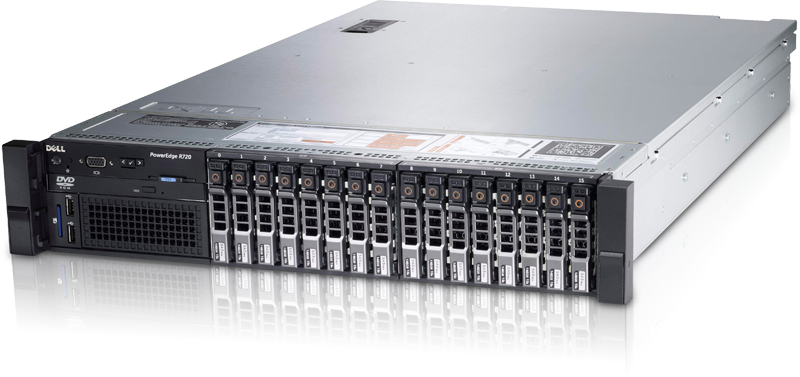
\includegraphics[width=6cm]{../figures/poweredge.png}
\end{center}
\end{frame}

\begin{frame}
So what kind of speed up to expect from threaded BLAS and LAPACK libraries.
\begin{center}
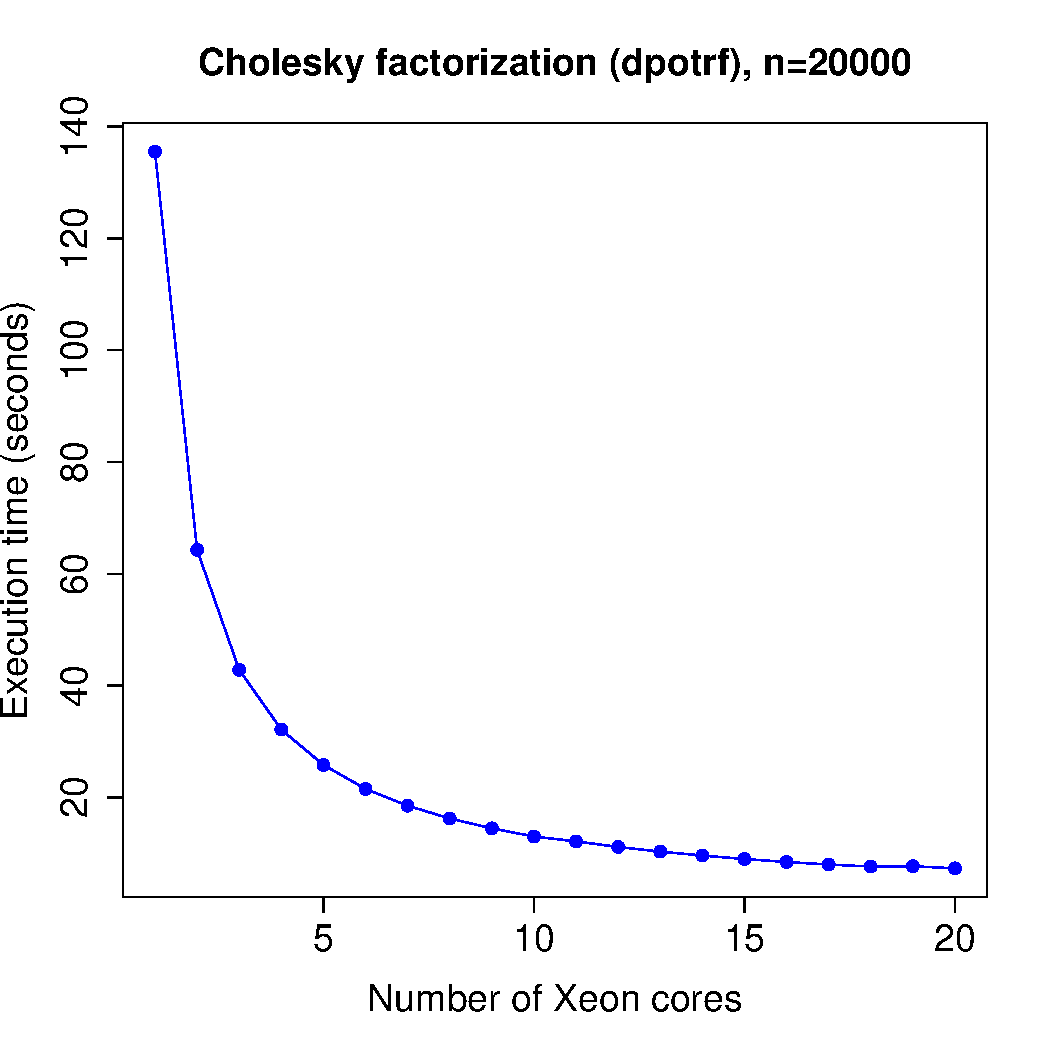
\includegraphics[width=5cm]{../figures/n20k-xeon.pdf}
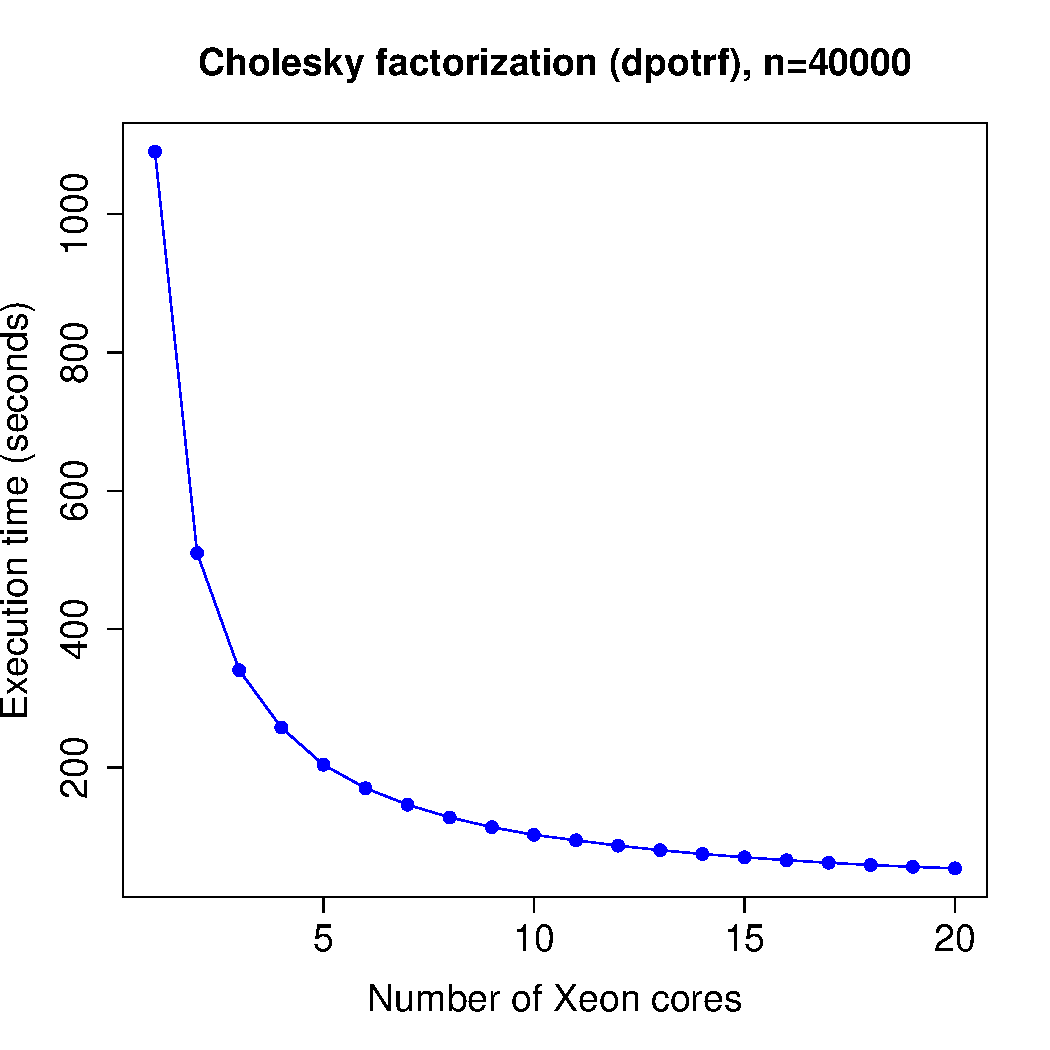
\includegraphics[width=5cm]{../figures/n40k-xeon.pdf}
\end{center}
\end{frame}

\begin{frame}
\begin{center}
\emph{R} and threaded BLAS and LAPACK
\end{center}

The BLAS and LAPACK that ``ships'' with \texttt{R} is single-threaded, but these can be replaced with multi-threaded libraries.

\begin{itemize}\setlength{\itemsep}{0.1cm}
\item[]\textbf{Windows}
  \begin{itemize}
  \item Microsoft \texttt{R} Open: The Enhanced \texttt{R} Distribution \url{https://mran.microsoft.com/open} comes with MLK \url{https://software.intel.com/en-us/mkl}.
  \item Replace existing \texttt{R}'s \texttt{libRblas.so} with OpenBLAS library \texttt{libopenblas.so}. OpenBLAS is available here \url{http://www.openblas.net}.
  \end{itemize}
\item[]\textbf{Max OS X}
  \begin{itemize}
  \item Mac vecLib obtained via XCode. Use install notes \href{https://cran.r-project.org/bin/macosx/RMacOSX-FAQ.html\#Which-BLAS-is-used-and-how-can-it-be-changed\_003f}{\beamergotobutton{here}}. 
  \end{itemize}
\item[]\textbf{Linux/Unix}
  \begin{itemize}
  \item MKL, OpenBLAS, ACML (compile \texttt{R} against MLK or post compile symbolic link of \texttt{libRblas.so} to \texttt{libopenblas.so}).
  \item Some additional gains using Intel icc and ifort compilers.
  \end{itemize}
\end{itemize}
\end{frame}

\end{document}
